\documentclass[12pt]{article} 
\usepackage[utf8]{inputenc}
\usepackage[T2A]{fontenc}
\usepackage{amsthm}
\usepackage{amssymb}
\usepackage{blindtext}
\usepackage{amsmath}
\usepackage{tikz} 
\usepackage{listings}
\usepackage{xcolor}
\usepackage{float}
\usepackage{graphicx}
\usepackage{hyperref}
\usepackage{wrapfig}
\hypersetup{
    colorlinks=true,
    linkcolor=blue,
    filecolor=blue,      
    urlcolor=blue,
    pdftitle={Overleaf Example},
    pdfpagemode=FullScreen,
    }
\graphicspath{ {./images} }

\title{Bioinformatics HW5}
\author{Ershov Ivan}
\date{May 2022}

\begin{document}
\maketitle
Я выбрал ген PTCH1
\paragraph{Задание 1.}
\subparagraph{1.а) Найдите выбранный ген в базе данных IntOGen. В каких типах рака он мутировал?\\}

Согласно сайту \href{https://www.intogen.org/search?gene=PTCH1}{IntOGen} выбранный ген мутировал в 6 типах:\\
\begin{enumerate}
    \item \href{https://www.intogen.org/search?cancer=SBCC}{Skin basal cell carcinoma}
    \item \href{https://www.intogen.org/search?cancer=MBL}{Medulloblastoma}
    \item \href{https://www.intogen.org/search?cancer=PIA}{Pilocityc astrocytoma}
    \item \href{https://www.intogen.org/search?cancer=ESCA}{Esophageal cancer}
    \item \href{https://www.intogen.org/search?cancer=OS}{Osteosarcoma}
    \item \href{https://www.intogen.org/search?cancer=MESO}{Mesothelioma}
\end{enumerate}
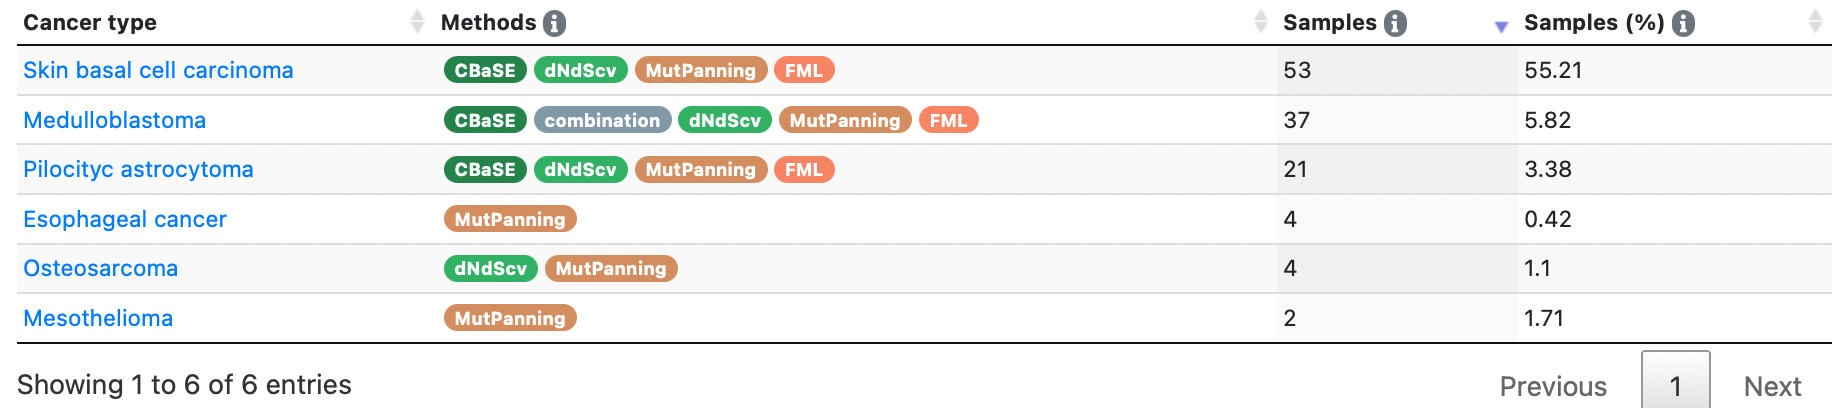
\includegraphics[width=\textwidth]{images/image1.png}\\\\
\subparagraph{1.б) Какие типы мутаций – точечные или структурные (вставки, делиции, транслокации)?\\}
Всего найдено 445 мутаций, среди которых встречаются как точечные, так и структурные:\\
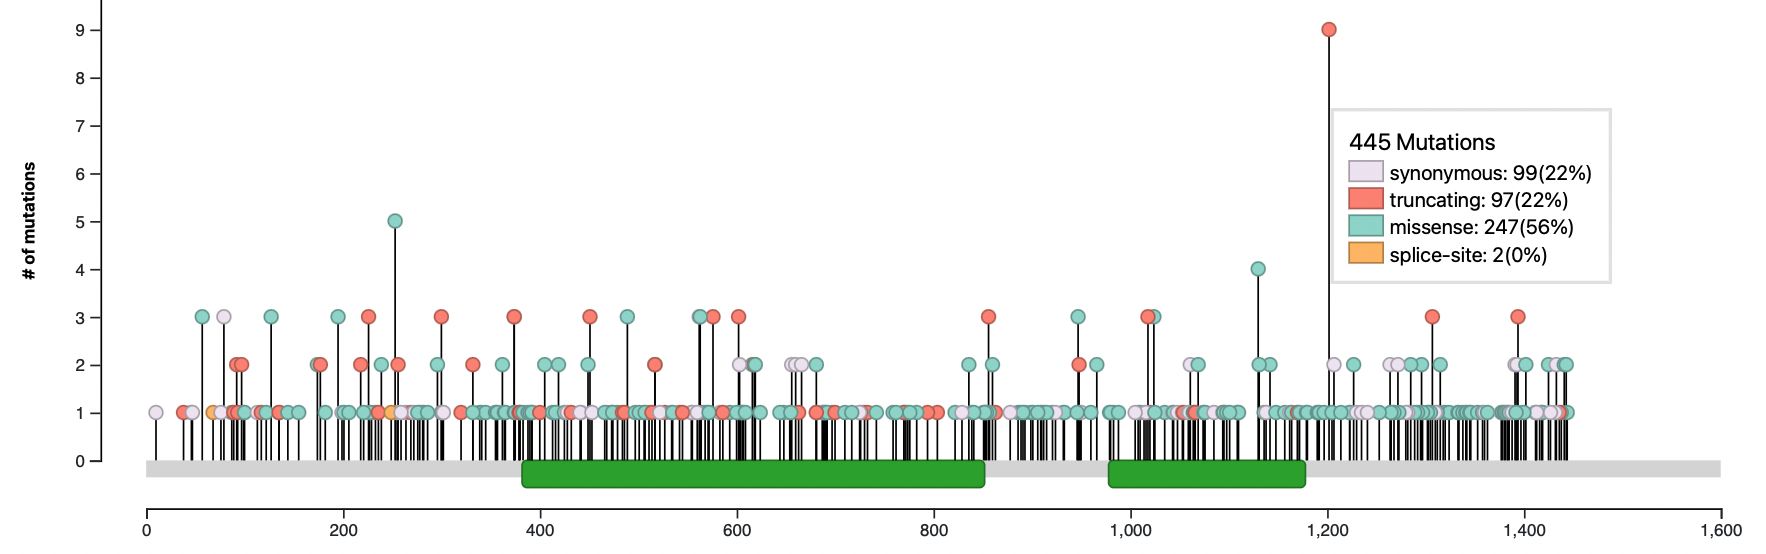
\includegraphics[width=\textwidth]{images/image2.png}\\\\
У данного гена есть как и вставки:\\
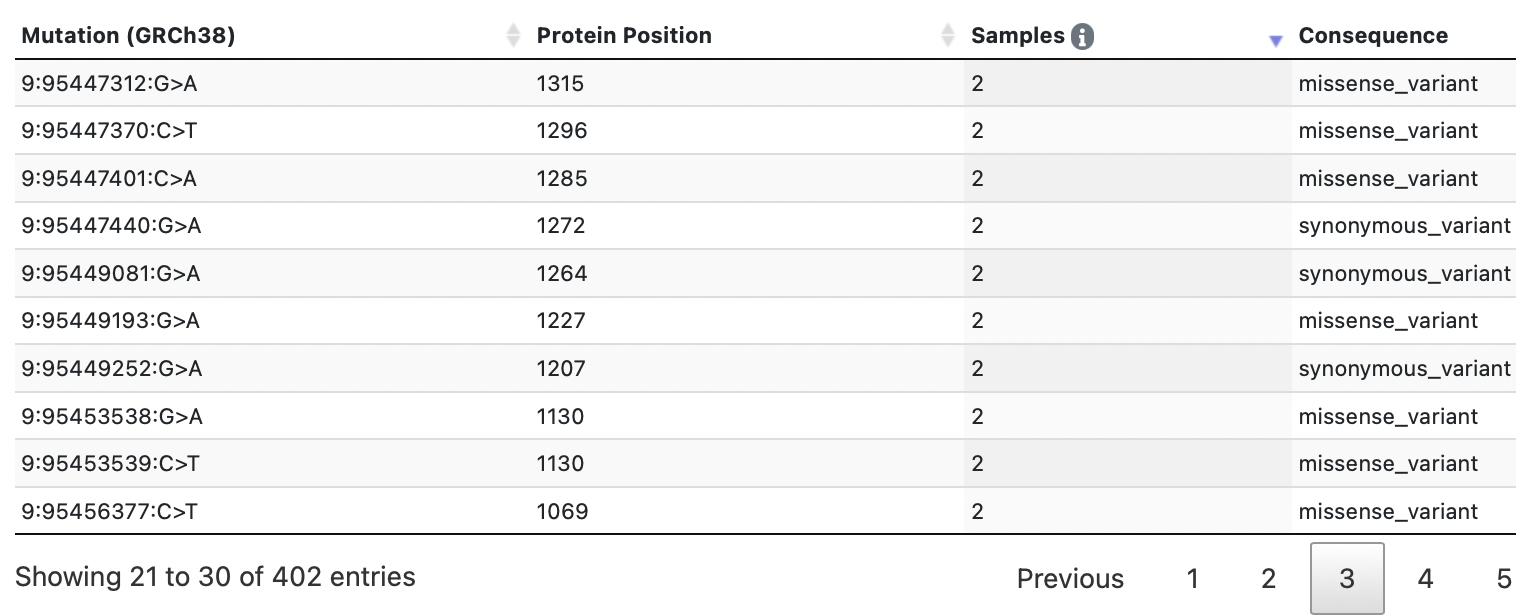
\includegraphics[width=\textwidth]{images/image3.png}\\\\
так и делиции:\\
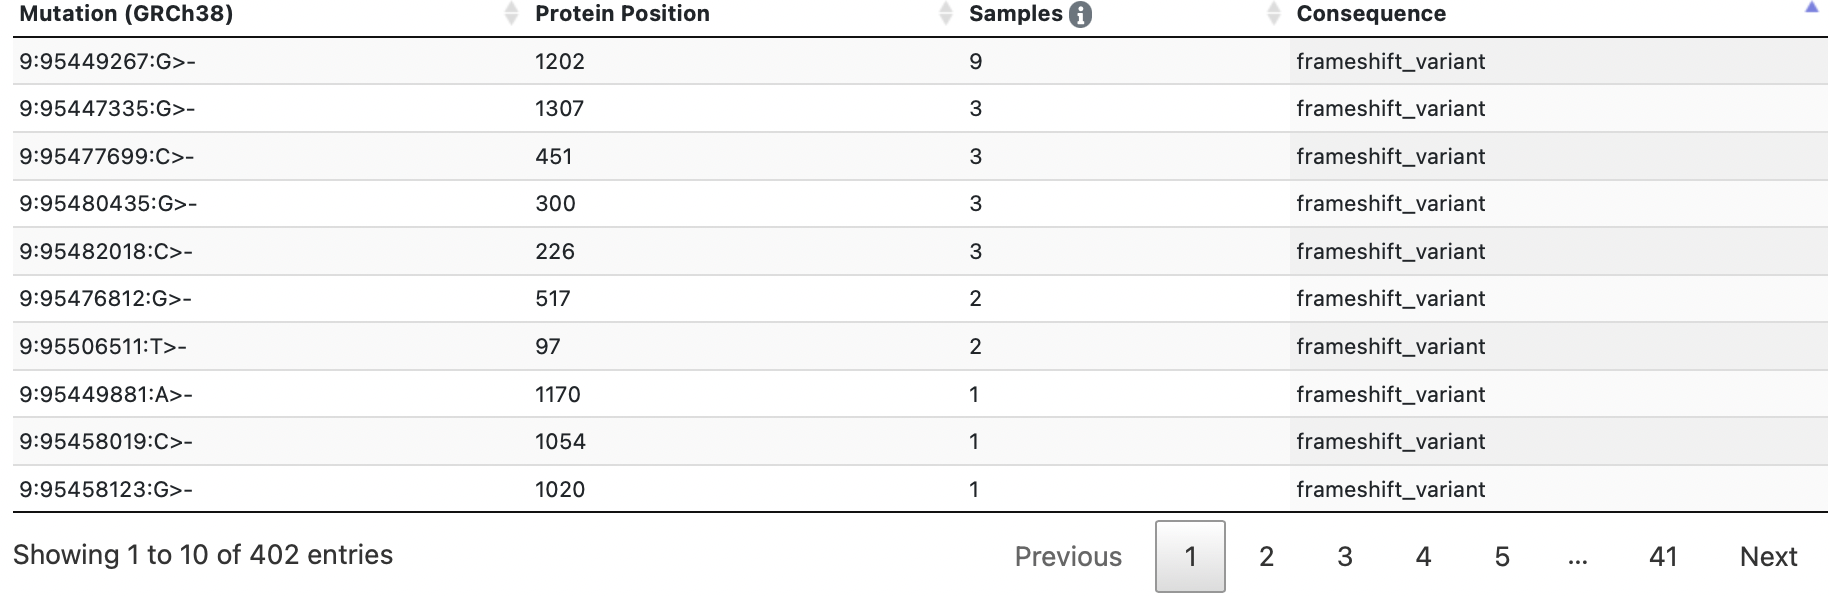
\includegraphics[width=\textwidth]{images/image4.png}\\\\

\subparagraph{2) Произведите поиск выбранного гена на портале ICGC: В каких типах рака выбранный ген мутирует?\\}
Смотрим на сайт \href{https://dcc.icgc.org/genes/ENSG00000185920/mutations?mutations}{ICGC}. На странице этого гена, есть две таблицы, в одной (таблица 1) отображены исследования различных типов рака с мутациями в данном гене, в другой (таблица 2) - представлена подробная информация о мутациях. В первой таблице в колонке Tumour Type как раз и написан тип рака:\\
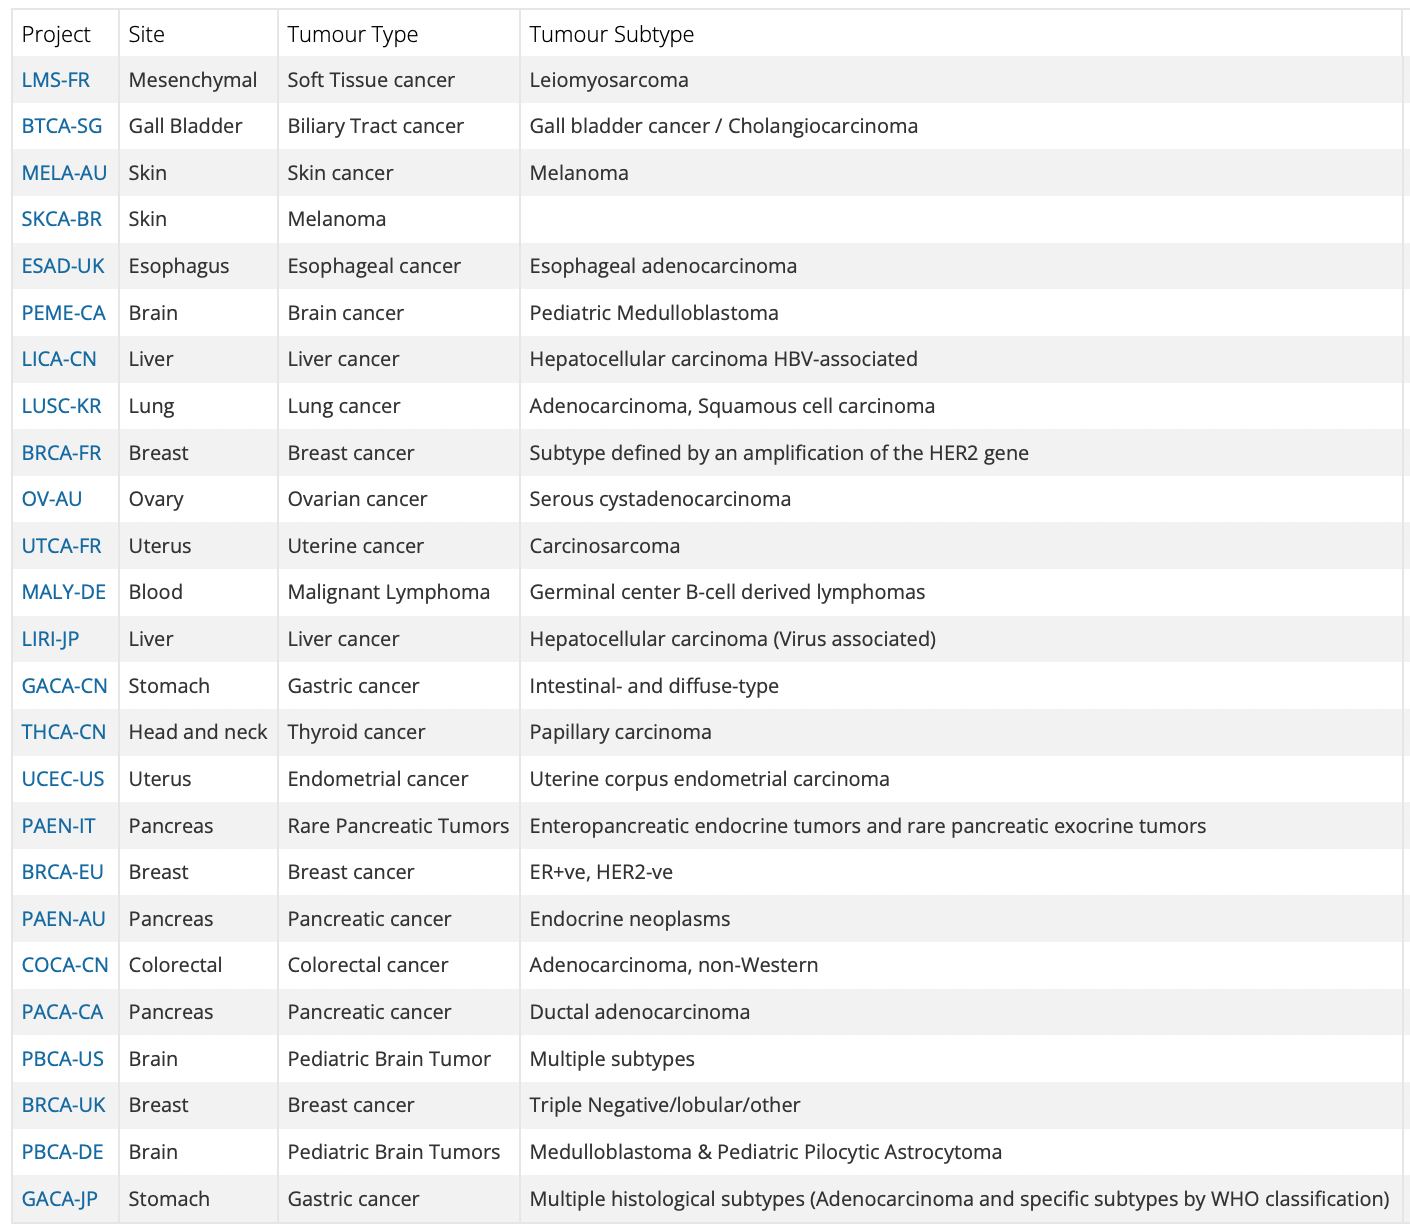
\includegraphics[width=\textwidth]{images/image5.png}\\\\
\pagebreak

\includegraphics[width=\textwidth]{images/image6.png}\\\\

\paragraph{Задание 2.\\}
\subparagraph{1)}
Выберем донора:
\begin{enumerate}
\setlength{\itemsep}{0pt}
    \item зайдем на сайт \href{https://dcc.icgc.org/genes/ENSG00000185920/mutations?mutations}{ICGC}
    \item выберем любой проект, например \href{https://dcc.icgc.org/projects/OV-AU}{OV-AU}
    \item перейдем на View in Data Repositories
    \item выберем любого донора, например \href{https://dcc.icgc.org/donors/DO46588}{DO46588}
\end{enumerate}

Проверим, действительно ли у этого человека мутация в нужном нам гене:
\begin{enumerate}
\setlength{\itemsep}{0pt}
    \item Скачаем с \href{https://dcc.icgc.org/donors/DO46588}{DO46588} "Simple Somatic Mutations" \href{https://dcc.icgc.org/genes/ENSG00000185920/mutations?mutations}{ICGC}
    \item поищем в скаченном файле \textbf{Ensembl ID}, соответсвующий гену (то есть ENSG00000185920, его я нашел \href{https://dcc.icgc.org/genes/ENSG00000185920}{тут})
\end{enumerate}
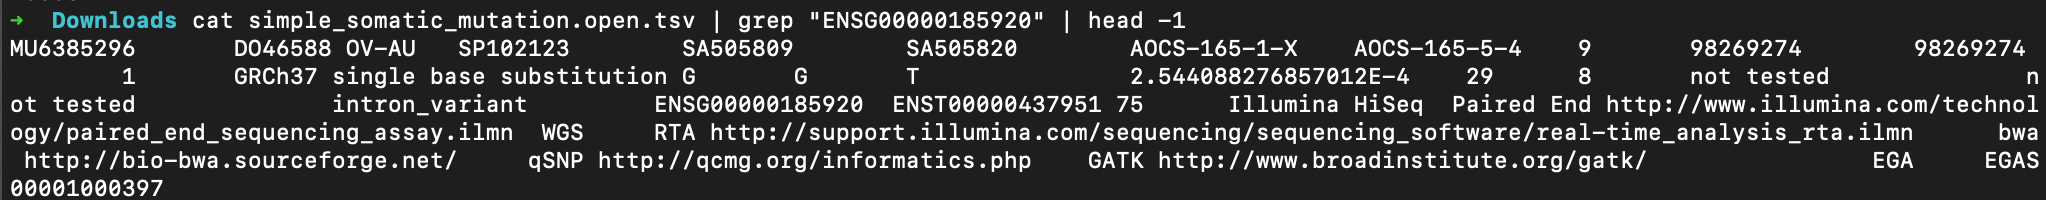
\includegraphics[width=\textwidth]{images/image7.png}\\\\
(тут очень много разной информации, но главное, что ENSG00000185920 нашелся, а значит, мутация была)
\pagebreak
\subparagraph{2)}
Теперь найдем еще 4 гена, с тем же типом рака, что и у нашего донора (то есть с Ovarian cancer):\\
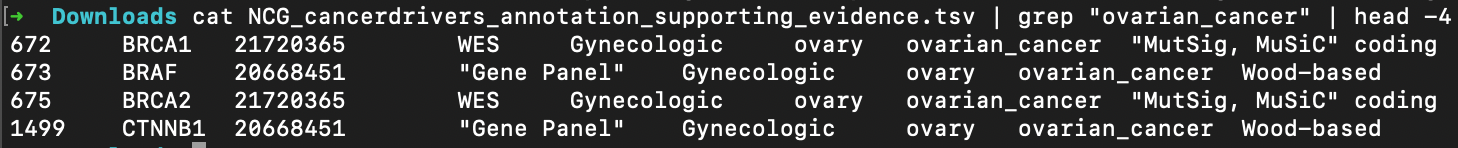
\includegraphics[width=\textwidth]{images/image8.png}\\\\
Найдем эти гены на сайте \href{https://dcc.icgc.org}{ICGC}:
\begin{enumerate}
    \item \href{https://dcc.icgc.org/genes/ENSG00000012048}{BRCA1}
    \item \href{https://dcc.icgc.org/genes/ENSG00000157764}{BRAF}
    \item \href{https://dcc.icgc.org/genes/ENSG00000139618}{BRCA2}
    \item \href{https://dcc.icgc.org/genes/ENSG00000168036}{CTNNB1}

\end{enumerate}
Теперь поищем мутации этих генов в выбранном доноре:\\
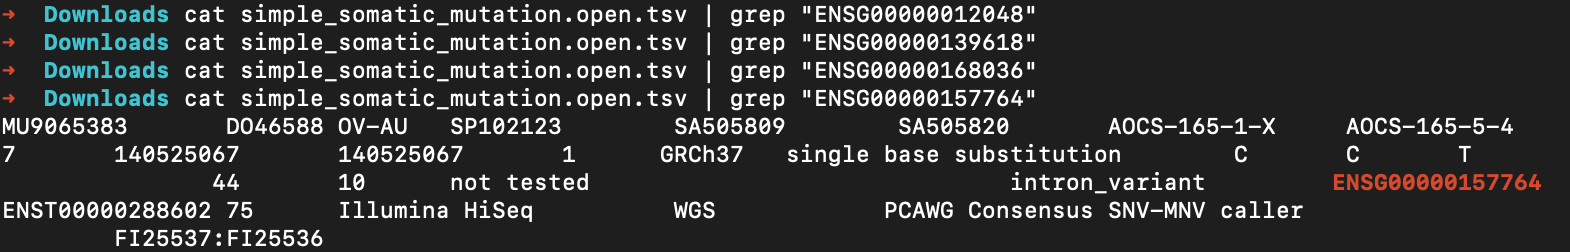
\includegraphics[width=\textwidth]{images/image9.png}\\\\
У данного донора рак яичников (Ovarian cancer). Поэтому стало интересно, обязательно ли должны произойти мутации в других генах, связанных с этим типом рака. Однако, как выяснилось, необязательно: среди выбранных 4 генов, ассоцируемых с раком яичников, только один мутировал.
\end{document}